\documentclass[a4paper,numbers=noenddot,abstract,DIV=calc]{scrartcl} %appendixprefix=true,chapterprefix=true
\usepackage[automark]{scrpage2} % para cabeçalhos
\usepackage{fontspec}
\defaultfontfeatures{Ligatures={TeX}}
\setmainfont{Minion Pro}
\setsansfont{Myriad Pro}
\setmonofont[Scale=.9]{Consolas}
\usepackage{polyglossia}
\setmainlanguage{brazil}
\setotherlanguages{french,english,german,russian,greek,spanish,italian,norsk}
\usepackage[tocgraduated]{tocstyle}
\usetocstyle{nopagecolumn}
\usepackage{graphicx}
\usepackage[marginal]{footmisc}
\usepackage{enumerate}
\usepackage[bookmarks]{hyperref}
\usepackage[dvipsnames]{xcolor}
\usepackage[xcolor]{mdframed}

\title{Título}
\author{Autor}
\date{Data}

\pagestyle{scrheadings} %retire se não quiser cabeçalhos

\begin{document}

\frenchspacing

\maketitle

\begin{abstract}
Escreva aqui o seu resumo. Escreva aqui o seu resumo. Escreva aqui o seu resumo. Escreva aqui o seu resumo. Escreva aqui o seu resumo. Escreva aqui o seu resumo.
\end{abstract}

\tableofcontents % comente ( % na frente) se não quiser sumário
\listoffigures % comente ( % na frente) se não houver figuras
%\listoftables % descomente (retire o %)se quiser lista de tabelas

%Use \% para porcento; \& para &. Dê espaço de uma linha entre dois parágrafos.
%Use \emph{texto} para itálico.
%Seja feliz.

\section{Coloque o título da seção}

\begin{figure}
\centering
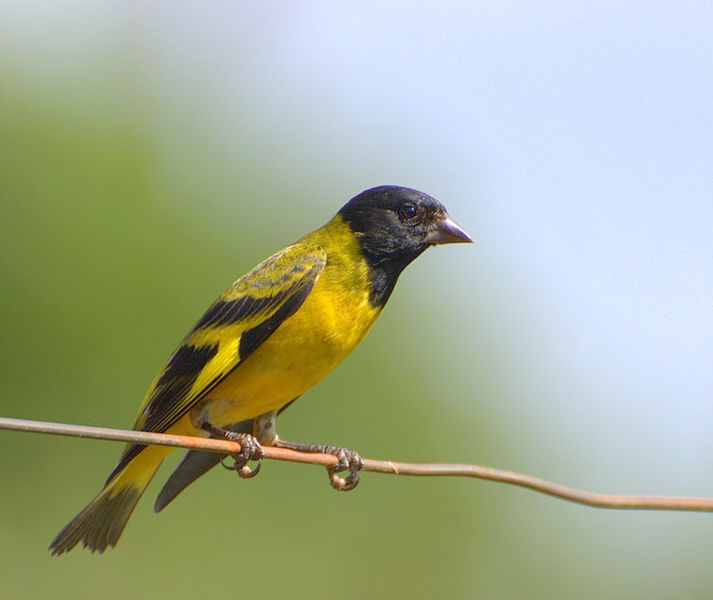
\includegraphics[width=0.5\linewidth]{pintassilgo}
\caption{Pintassilgo-de-cabeça-preta. \textit{Carduelis magellanica}.}
\label{pintassilgo}
\end{figure}



\section{Coloque o título da seção}

\section{Coloque o título da seção}

\section*{Bibliografia}
\addcontentsline{toc}{section}{Bibliografia}

\setlength{\parindent}{0pt}

Schimmel, Annemarie, and Stuart Cary Welch. \textit{Anvari's Divan: A Pocket Book for Akbar}.  New York: The Metropolitan Museum of Art, 1983.

\setlength{\parskip}{10pt} %acrescente depois da primeira entrada bibliográfica

Mearsheimer, John. \textit{The Tragedy of Great Power Politics.} New York and London: W.W. Norton \& Company, 2001.




\end{document}
